\documentclass[12pt]{article}

\usepackage{amsmath}
\usepackage{amssymb}
\usepackage{listings}

\usepackage[explicit]{titlesec}
\usepackage{titletoc}
\usepackage{fancyhdr}

%%\usepackage{wrapfig}
%%\usepackage{caption}

\usepackage{xcolor}
\usepackage{graphicx}
%%\usepackage{textcase}
\usepackage[margin=1.5cm]{caption}
\usepackage{mathptmx}

%%\usepackage[hidelinks]{hyperref}
\usepackage{hyperref}
\usepackage{enumitem}
\usepackage{parskip}
\usepackage[backend=bibtex]{biblatex}
\usepackage[margin=0.5in]{geometry}

\makeatletter

%%\DeclareCaptionFormat{hrformat}{#1#2#3\vspace{-5pt}{\color{darkgray}\hrulefill}\vspace{25pt}}
%%\captionsetup[figure]{format=hrformat}
\setlist{leftmargin=1.4em,nosep}
\renewcommand\labelitemi{--}

\newcommand{\headline}[2]{\textbf{#1}: #2\\}

\newcommand{\examno}[1]{\gdef\@examtitle{Exam #1\\}}
\newcommand{\prjctno}[1]{\gdef\@examtitle{Project #1\\}}
\newcommand{\examtitle}[1]{\gdef\@examtitle{#1\\}}
\newcommand{\student}[1]{\gdef\@student{#1}}
\newcommand{\course}[1]{\gdef\@course{#1}}
\newcommand{\due}[1]{\gdef\@due{#1}}


\newcommand{\@examtitle}{Exam ?\\}
\newcommand{\@student}{Joe Opseth}
\newcommand{\@course}{Applied Regression Analysis}
\newcommand{\@due}{\today}

\titleformat{\section}
  [hang]
  {\normalfont\large\bfseries}
  {\thesection}
  {1em}{}

\titleformat{\subsection}
  [hang]
  {\normalfont\small\bfseries}
  {\thesubsection}
  {1em}{}


\renewcommand{\maketitle}{\noindent
  \@student\\
  \@due\\
  %% \headline{Name}{\@student}
  %% \headline{Course}{\@course}
  %% \headline{Date}{\@due}
  {\par\centering\LARGE\@examtitle\par}
}

\newcommand\mytodo[1]{\textcolor{red}{(TODO: #1)}}
%% To remove all TODOs, uncomment this line:
%% \renewcommand\mytodo[1]{}

\newcommand\ts{\thicksim}
\newcommand\mr[1]{\mathrm{#1}}
\newcommand\eqnone{\\ \hspace*{1cm} (1)}
\newcommand\eqntwo{\\ \hspace*{1cm} (2)}
\newcommand\distf[2]{\ensuremath{\mr{#1}(#2)}}
\newcommand\thetaone{\ensuremath{\hat{\theta_1}}}
\newcommand\thetatwo{\ensuremath{\hat{\theta_2}}}

\pagestyle{headings}
\addtolength{\headheight}{\baselineskip}
\fancyhf{}
\fancyhead[L]{\rightmark}
\fancyhead[R]{\thepage}
\fancypagestyle{plain}{% Redefine plain pages tyle
  \fancyhf{}% Clear header/footer
  \renewcommand{\headrulewidth}{0.0pt}%
  \fancyhead[R]{\thepage}
}

%% \sl for slant
%% \sl needs to be before \sffamily or it clobbers the font selection
%% If a period is desired after all captions, this can be modified with a period
%%\scriptsize a little bit smaller than \footnotesize
\newcommand\nocaption[1]{\newline\footnotesize\sffamily #1}

%%% Commands for section subtitles
%%% See https://tex.stackexchange.com/a/102682
%%% Usage: 
%%
%% \sectiondate{March 15, 2013}
%% \sectionsubtitle{Test Subtitle}
%% \section{Test Section With a Title Spanning Two Lines}
%% \lipsum[4]

%% \undefds
%% \section{Test Section}
%% \lipsum[4]

\newcommand*\nameundef[1]{%
  \expandafter\let\csname #1\endcsname\@undefined}
\newcommand\sectiondatefont{\normalfont\rmfamily\itshape\bfseries\Large}
\newcommand\sectionsubtitlefont{\normalfont\rmfamily\it\normalsize}
\newcommand\sectiondate[1]{\def\@sectiondate{#1}}
\newcommand\sectionsubtitle[1]{\def\@sectionsubtitle{#1}}
\titleformat{\section}
  {\normalfont\large\rmfamily}{}{0em}
  {\colorbox{white}{%
    \parbox[t]{\dimexpr\textwidth-2\fboxsep-2\fboxrule\relax}{%
      \vspace*{1ex}%
      \@ifundefined{@sectiondate}
        {}{{\sectiondatefont\@sectiondate}\\*}%
      \raggedright%
      \textcolor{black}{\Large{#1}}%
      \@ifundefined{@sectionsubtitle}
        {}{\\*\textcolor{darkgray}{\sectionsubtitlefont\@sectionsubtitle}}%
      \vspace*{1ex}
      }%
    }%
  }
\newcommand\undefds{%
  \nameundef{@sectiondate}\nameundef{@sectionsubtitle}}




\makeatother

\bibliography{publications}

\begin{document}

\thispagestyle{empty}

\examtitle{Project Portfolio}
%% \course{Mathematical Statistics}




\maketitle

\sectionsubtitle{Object-Oriented Programming, University of Wisconsin-River Falls}
\section*{Exam Builder}%
\markboth{Exam Builder}{Exam Builder}

A Java application that builds exams from a pool of questions stored in a text file. Includes a GUI and text-based interface. Questions may be multiple choice, short answer, or long answer, and the exam generated can be customized for the number of questions to use and the range of chapters to pull from. 

\paragraph{Skills Used}
\begin{itemize}
\item Java
\item JUnit
\item Java Collections
\item Eclipse
\item IntelliJ Idea
\end{itemize}

\vspace{\baselineskip}
Github: \url{https://github.com/joe-op/course-project}

\vspace{20pt}

\begin{figure}[ht]
\centering
    \makebox[\textwidth][c] {
      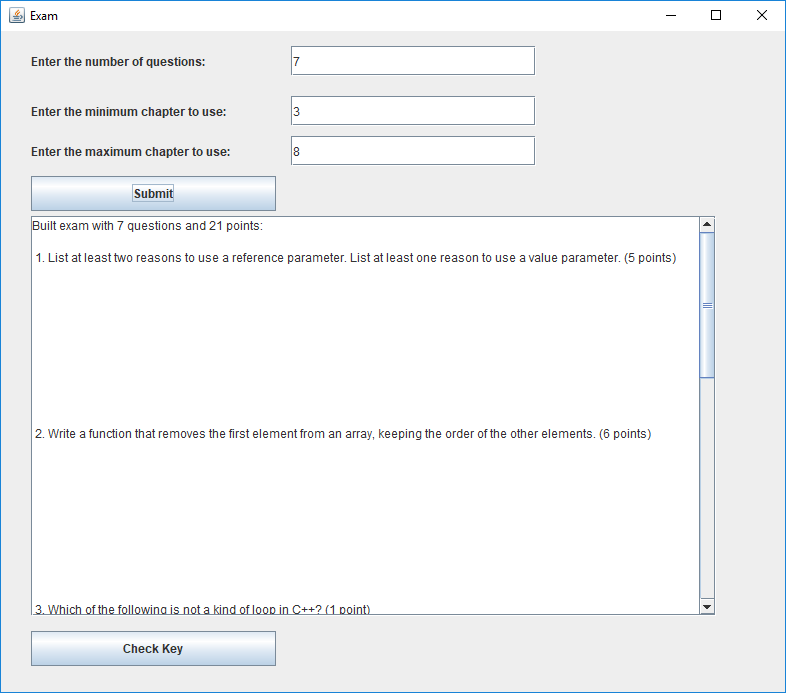
\includegraphics[width=0.6\textwidth]{images/exam-builder-01}
    }
    \nocaption{GUI showing generated exam}
    \label{fig:exam-1}
\end{figure}
\begin{figure}
\centering
    \makebox[\textwidth][c] {
      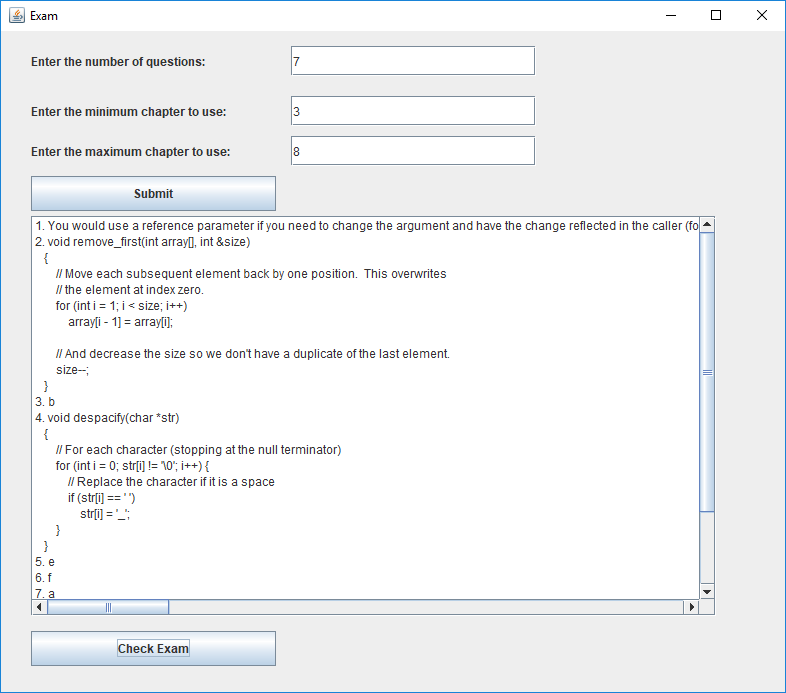
\includegraphics[width=0.6\textwidth]{images/exam-builder-02}
    }
    \nocaption{GUI showing exam key}
    \label{fig:exam-2}
\end{figure}
\begin{figure}
\centering
    \makebox[\textwidth][c] {
      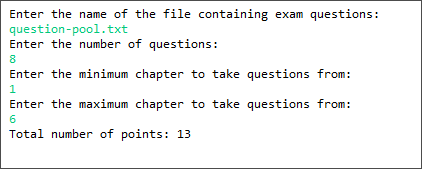
\includegraphics[width=0.5\textwidth]{images/exam-builder-03}
    }
    \nocaption{Text interface for outputting exam to file}
    \label{fig:exam-3}
\end{figure}


\clearpage

\sectionsubtitle{Data Structures and Algorithms, University of Wisconsin-River Falls}
\section*{C++ Database Implementation}
\markboth{C++ Database Implementation}{C++ Database Implementation}
\thispagestyle{plain}

Collaborated on a program that implemented a simple database in C++ with insert, find, and delete features.  The database used a binary search tree to find records and included a primary key and a secondary index.

\paragraph{Skills Used}
\begin{itemize}
\item C++
\item Algorithms
\item Pointers
\item Visual Studio
\end{itemize}


\vspace{\baselineskip}
Github: \url{https://github.com/joe-op/237-PA4}
\vspace{20pt}

\begin{figure}[ht]
  \centering
  \makebox[\textwidth][c] {
    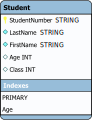
\includegraphics[width=0.35\textwidth]{images/rdb-02}
  }
  \nocaption{Diagram of the Student table that was implemented using the database system}
    \label{fig:rdb-2}
\end{figure}
\begin{figure}
\centering
    \makebox[\textwidth][c] {
      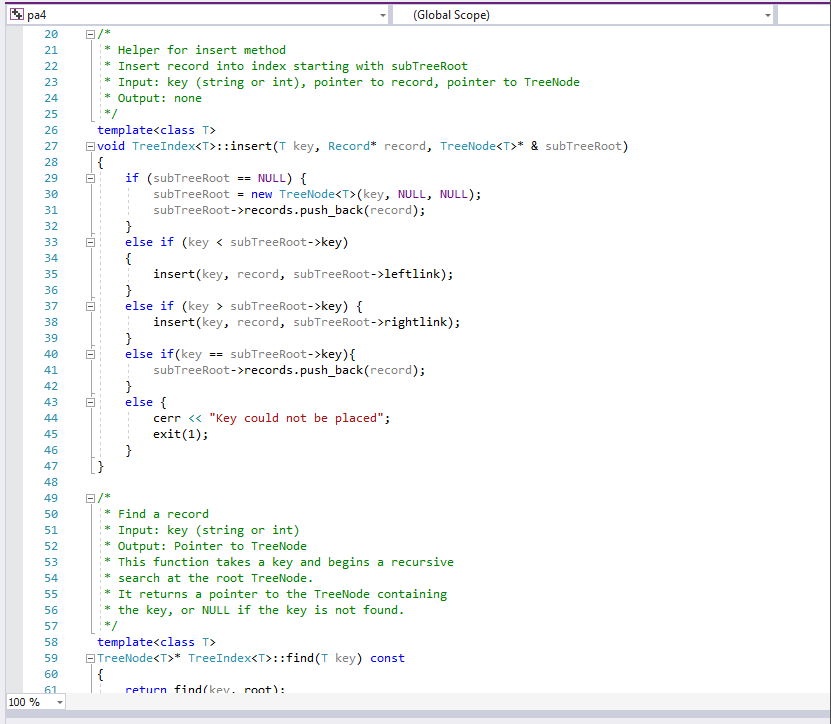
\includegraphics[width=0.6\textwidth]{images/rdb-01}
    }    
    \nocaption{The database used a binary search tree to find records}
    \label{fig:rdb-1}
\end{figure}
\begin{figure}
\centering
    \makebox[\textwidth][c] {
      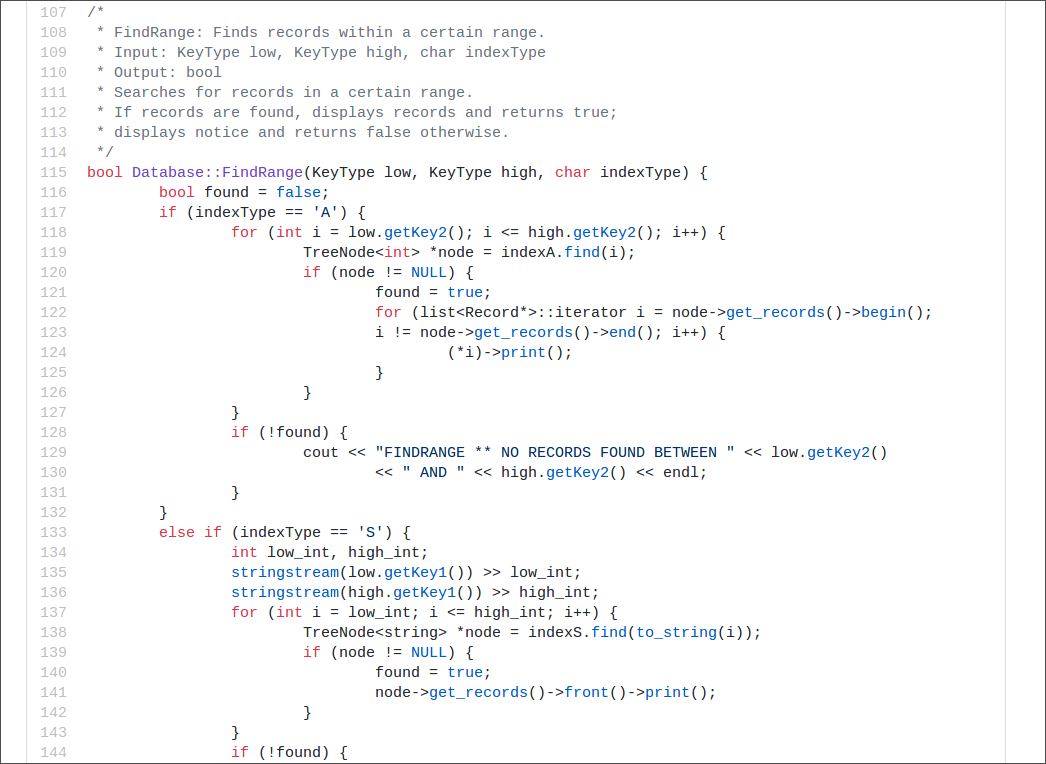
\includegraphics[width=0.6\textwidth]{images/rdb-03}
    }
    \nocaption{Indices were made on StudentNumber and Age}
    \label{fig:rdb-3}
\end{figure}

\clearpage

\sectionsubtitle{Database Management Systems, University of Wisconsin-River Falls}
\section*{Stock Management Web Application}
\markboth{Stock Management Web Application}{Stock Management Web Application}
\thispagestyle{plain}
    
Collaborated on a web application for internal use of a stock management company.  The application was written using PHP.  We used SQL queries to retrieve information on agents, clients, companies, and stock reports, and we used the Ruby gem Faker to generate some of the data used to demonstrate the application.  The application retrieved and displayed various reports and provided CRUD web forms for entities such as agents, companies, and headquarters. 

\paragraph{Skills Used}
\begin{itemize}
\item MySQL
\item PHP
\item HTML
\item CSS
\item Apache
\item MariaDB
\end{itemize}


\vspace{\baselineskip}
Github: \url{https://github.com/joe-op/333-CourseProject}

\begin{figure}[ht]
\centering
    \makebox[\textwidth][c] {
      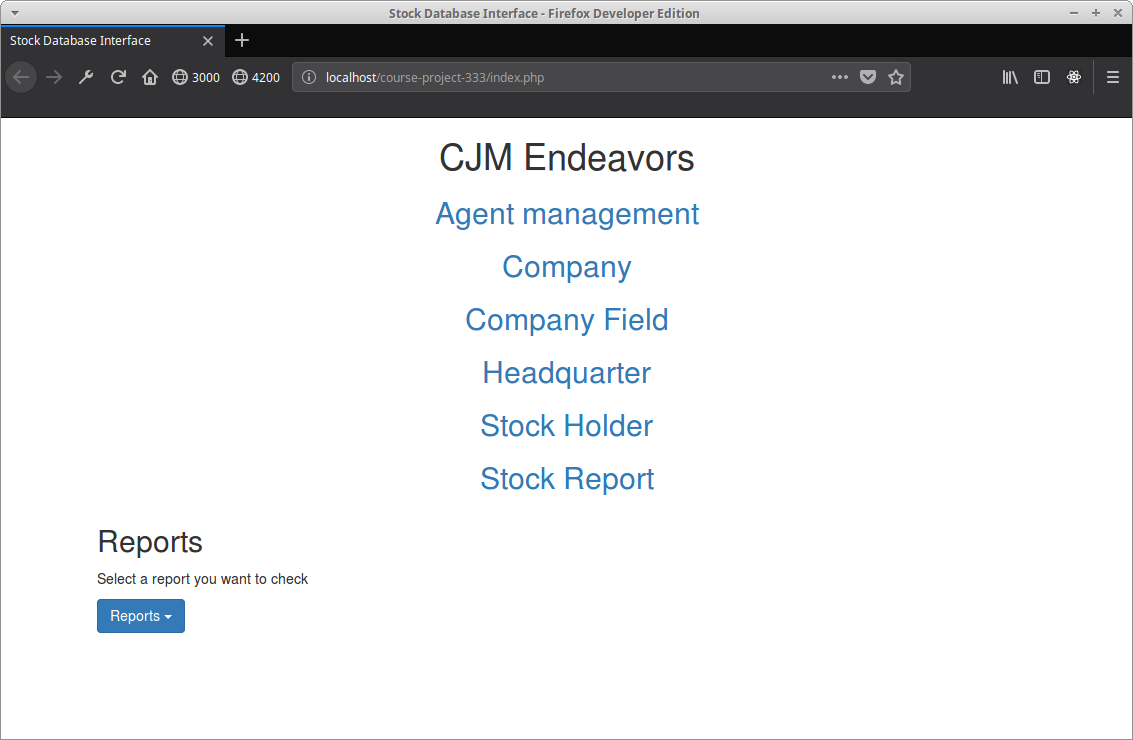
\includegraphics[width=0.6\textwidth]{images/stock-01}
    }
    \nocaption{The application provides an interface for managing the company's database.  Also provided are various reports built from custom SQL queries}
    \label{fig:exam-1}
\end{figure}

\begin{figure}
\centering
    \makebox[\textwidth][c] {
      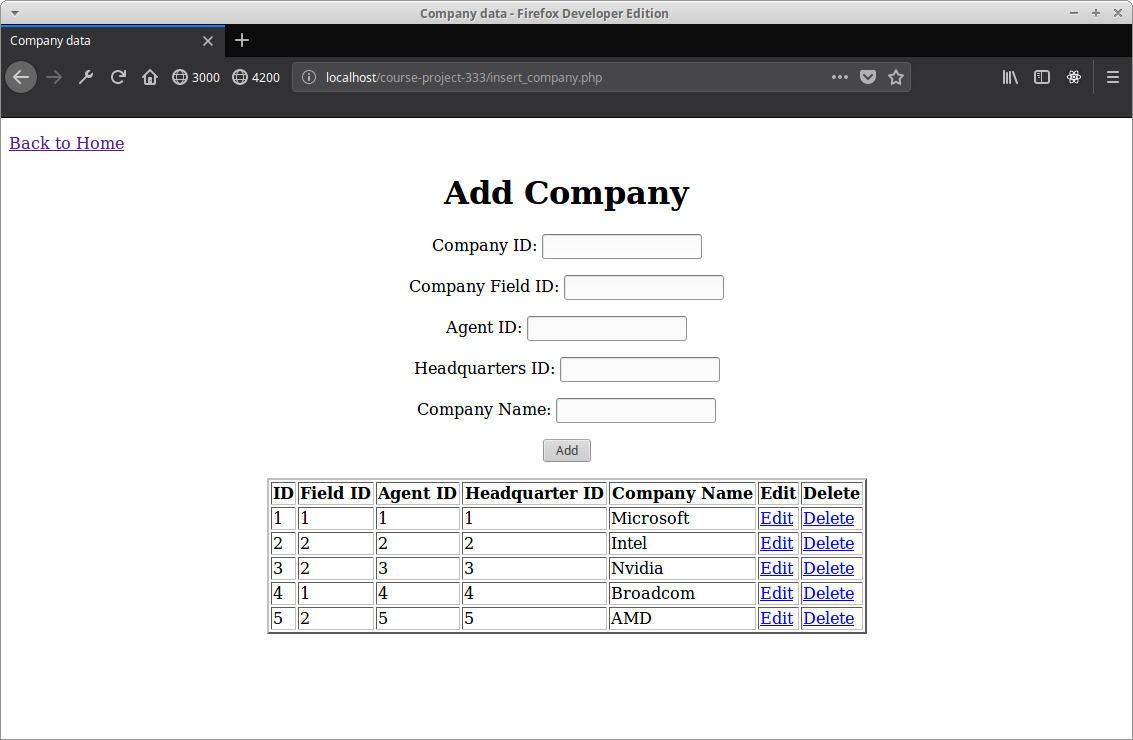
\includegraphics[width=0.6\textwidth]{images/stock-02}
    }
    \nocaption{Provides CRUD functionality for records}
    \label{fig:exam-2}
\end{figure}

\begin{figure}
\centering
    \makebox[\textwidth][c] {
      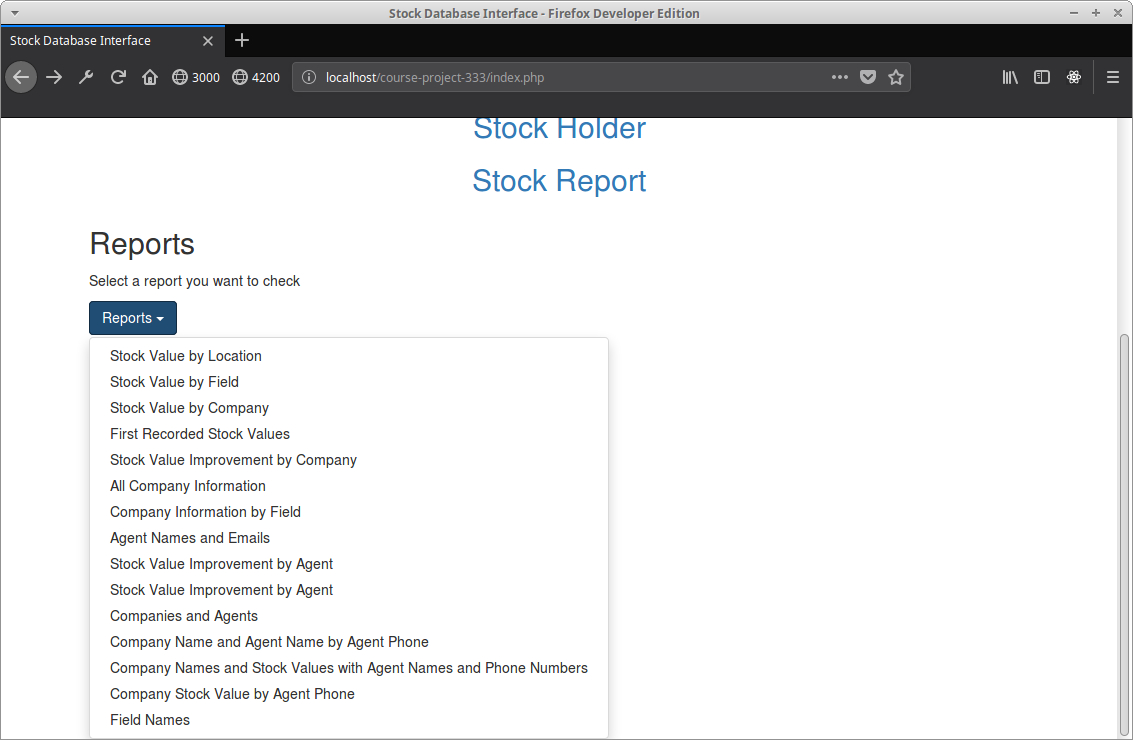
\includegraphics[width=0.6\textwidth]{images/stock-04}
    }
    \nocaption{Users can access various reports pulled from the database}
    \label{fig:exam-4}
\end{figure}

\begin{figure}
\centering
    \makebox[\textwidth][c] {
      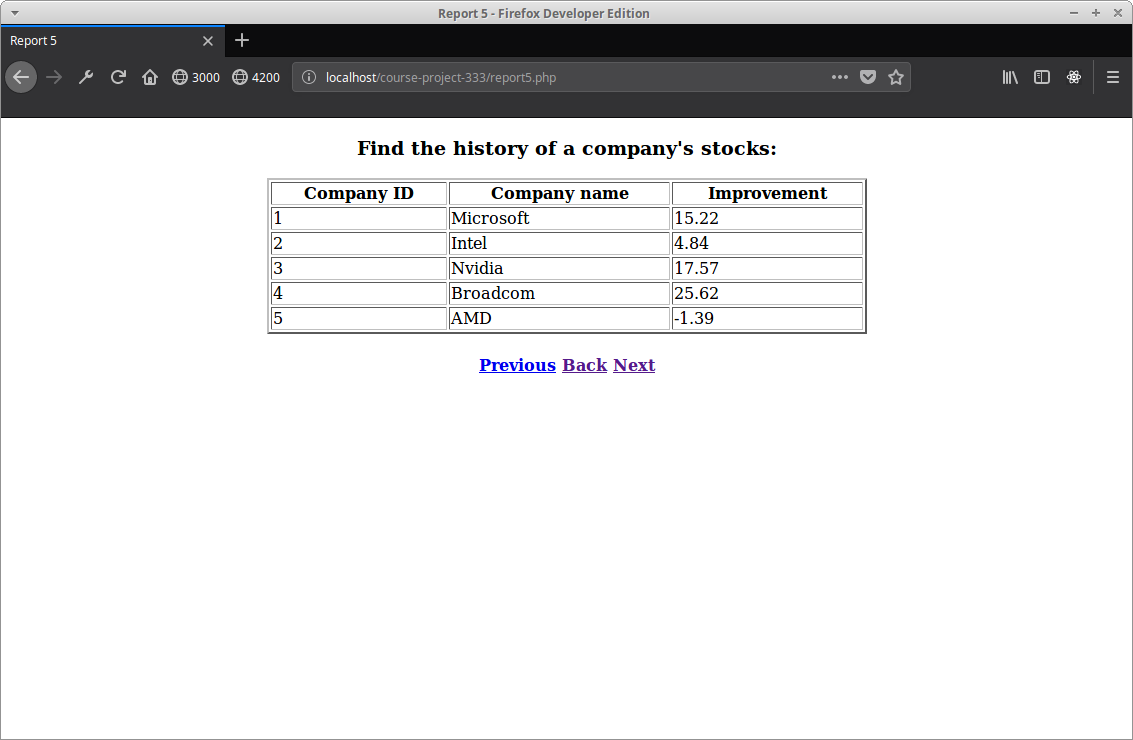
\includegraphics[width=0.6\textwidth]{images/stock-03}
    }
    \nocaption{A report showing the improvement in each company's stocks}
    \label{fig:exam-3}
\end{figure}

\clearpage

\sectionsubtitle{Full Stack Web and Multiplatform Mobile App Development\\\vspace{-5pt}The Hong Kong University of Science and Technology through Coursera}
\section*{Restaurant Website}
\markboth{Restaurant Website}{Restaurant Website}
\thispagestyle{plain}

A website for a restaurant, including the restaurant's menu, information on the corporate leaders, and contact information.  In the specialization's first course -- Bootstrap 4 -- we built the user interface using Node.js with Bootstrap and FontAwesome modules.  Features included modals for logging in and reserving a table, a responsive navigation bar that collapses into a dropdown menu for mobile devices, a carousel on the home page for featuring items, and stylized contact and social media links.

In the second course we are redesigning the site using Angular.  The UI framework has been switched from Bootstrap to Material Design, and elements such as menu items and corporate leaders have been rewritten as TypeScript objects provided by services, allowing the HTML templates and the objects to be more easily updated and expanded.  

\paragraph{Skills Used}
\begin{itemize}
\item JavaScript \& TypeScript
\item Node.js \& NPM
\item Angular Framework
\item Chrome \& Firefox developer tools
\item CSS preprocessors
\item Gulp \& Grunt taskrunners
\item HTML5 \& CSS3
\item Bootstrap
\item Angular Flex Layout
\item Angular Material Design
\end{itemize}

%%\subsection*{Favorite Parts of the Project}

%% \begin{figure}
%%   \centering
%%   \makebox[\textwidth][c] {
%%     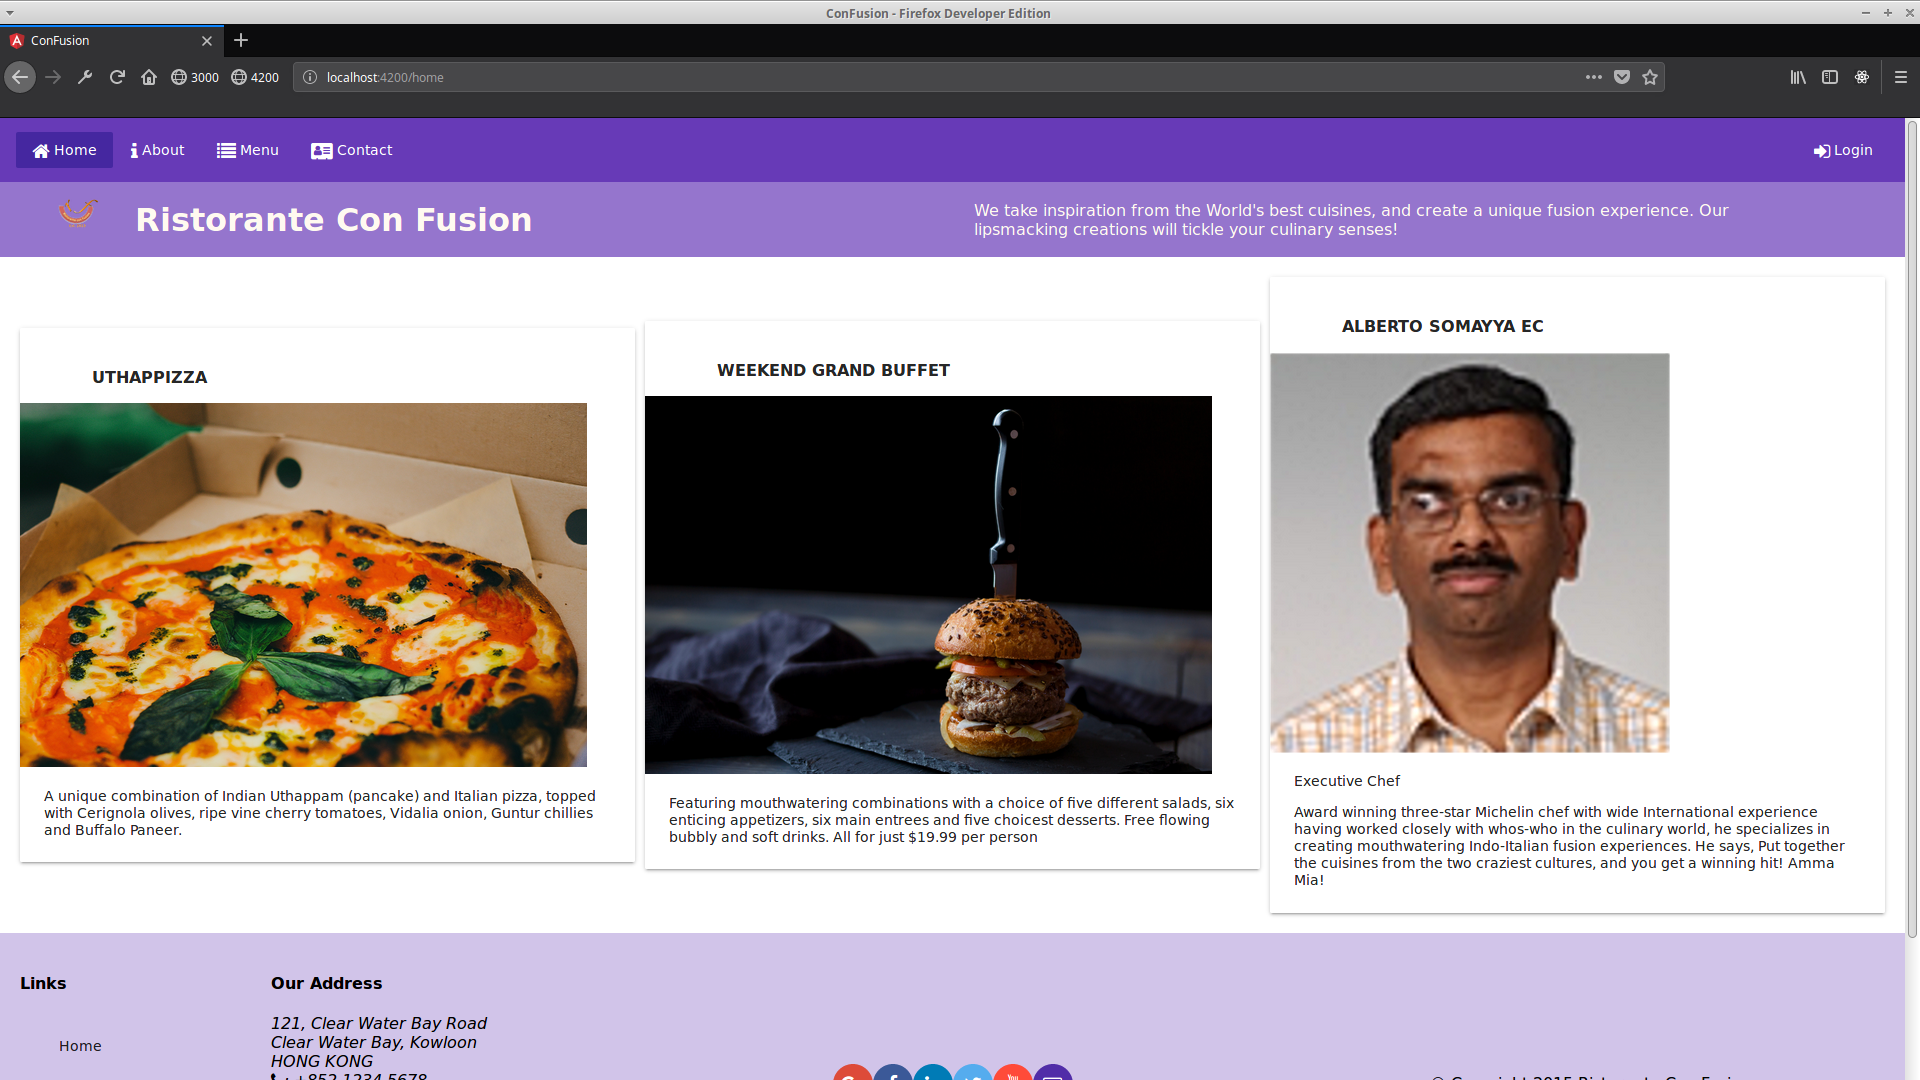
\includegraphics[width=0.6\textwidth]{images/ristorante-01}
%%   }
%%   \nocaption{}
%%   \label{fig:ristorante-1}
%% \end{figure}

\begin{figure}[ht]
  \centering
  \makebox[\textwidth][c] {
    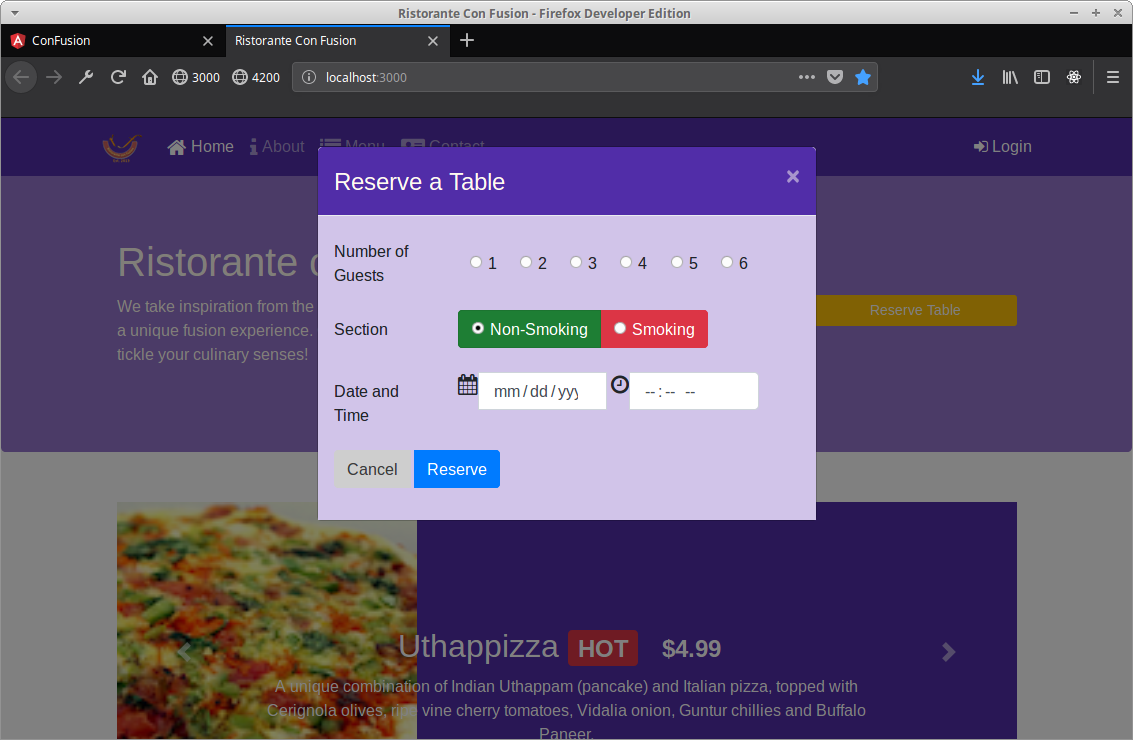
\includegraphics[width=0.6\textwidth]{images/ristorante-03}
  }
  \nocaption{A modal for making a reservation}
  \label{fig:ristorante-3}
\end{figure}

\begin{figure}
  \centering
  \makebox[\textwidth][c] {
    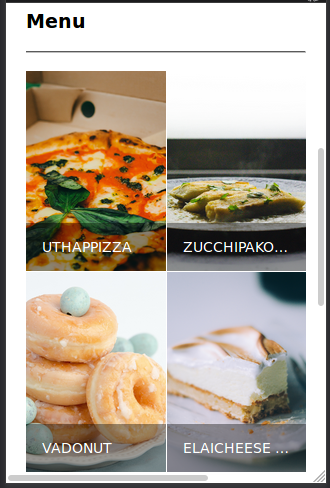
\includegraphics[width=0.3\textwidth]{images/ristorante-02}
  }
  \nocaption{The mobile view of the restaurant's menu}
  \label{fig:ristorante-2}
\end{figure}

\begin{figure}
  \centering
  \makebox[\textwidth][c] {
    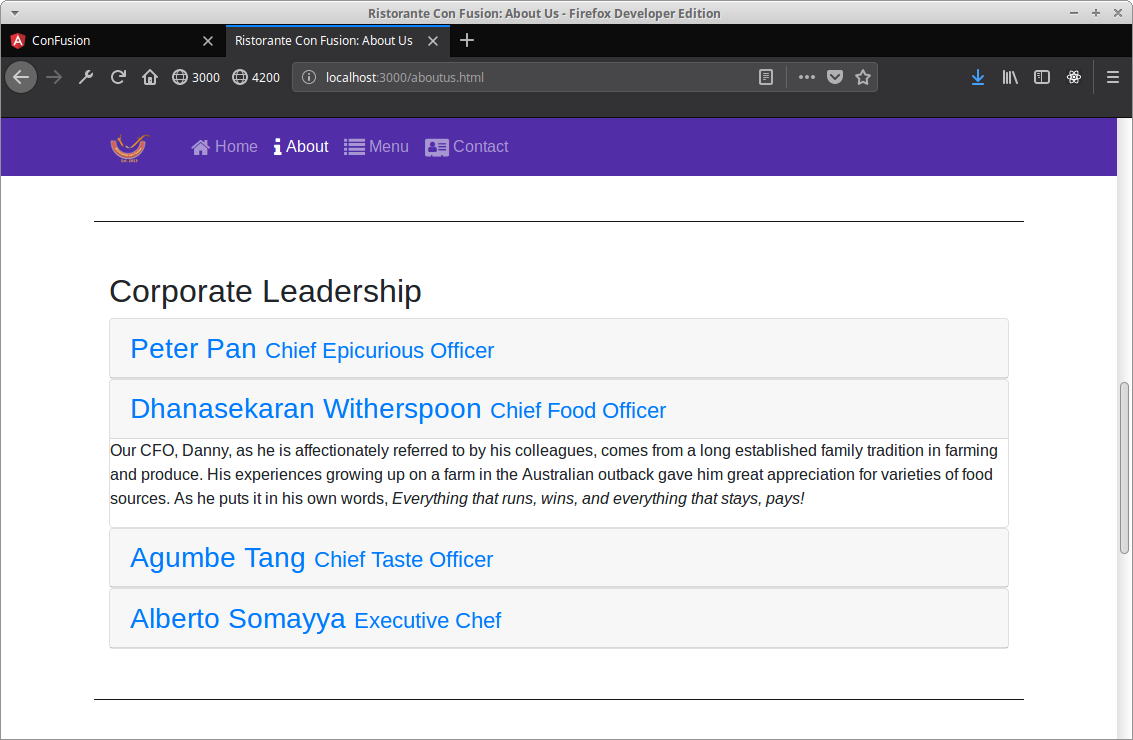
\includegraphics[width=0.6\textwidth]{images/ristorante-04}
  }
  \nocaption{A Bootstrap accordion showing information about the corporate leaders}
  \label{fig:ristorante-4}
\end{figure}

%% \begin{figure}
%%   \centering
%%   \makebox[\textwidth][c] {
%%     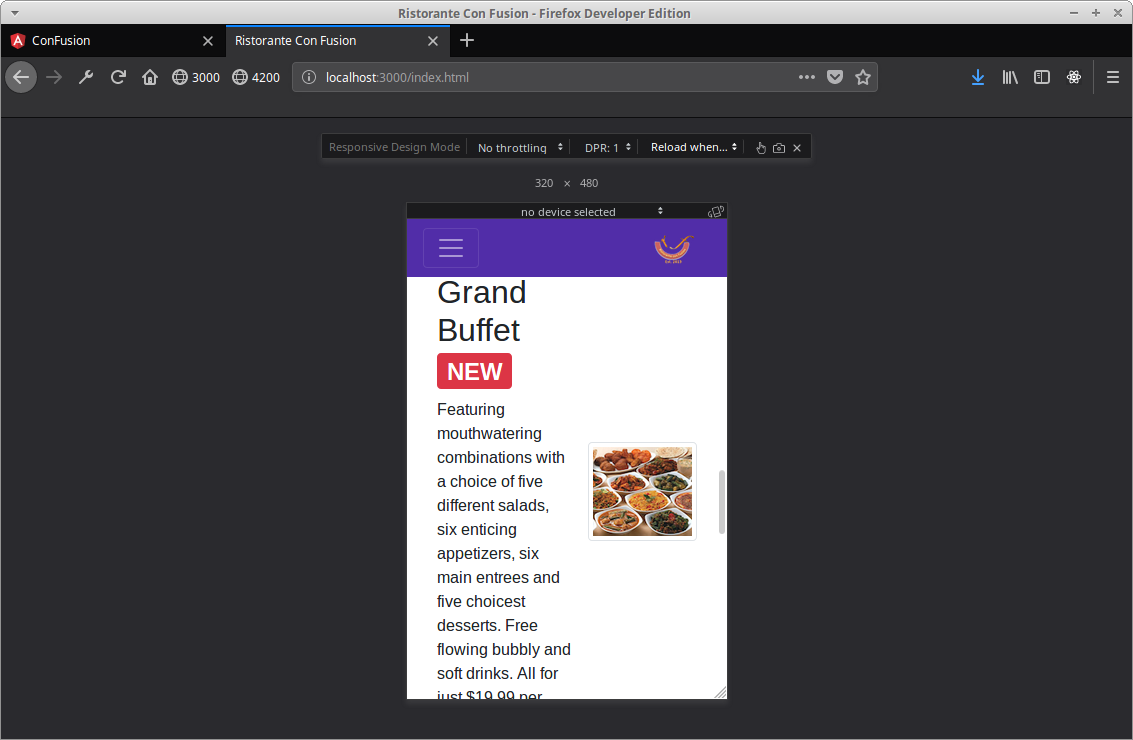
\includegraphics[width=0.6\textwidth]{images/ristorante-05}
%%   }
%%   \nocaption{The navigation bar and home page items scaled for mobile}
%%   \label{fig:ristorante-5}
%% \end{figure}

\clearpage
\sectionsubtitle{University of Wisconsin-River Falls}
\section*{Self-assembly Research}
\markboth{Self-assembly Research}{Self-assembly Research}
\thispagestyle{plain}

The field of self-assembly is motivated by the fact that DNA molecules can be designed in such a way that, when they are combined, they will autonomously form into ``assemblies'' whose structure is determined by the design of the molecules.  Research in this field ranges from wet-lab work with DNA, to designing mathematical models based on the properties of DNA, to abstract mathematical research exploring the limits of these models.  Our research in the last category concerned the possibility or impossibility of certain types of constructions in the 2HAM and STAM models of self-assembly. One result~\cite{4sided} shows that any fractal that belongs to a class of fractals we call ``4-sided'' can be strictly self-assembled in the 2HAM, while the same is not true for ``3-sided'' fractals (that is, there exists a 3-sided fractal that cannot be strictly self-assembled in the 2HAM).

A comprehensive introduction to the field of self-assembly can be found at the self-assembly wiki: \url{http://self-assembly.net}.

\paragraph{Skills Used}
\begin{itemize}
\item Mathematical Modeling
\item Mathematical Writing 
\item Figure design with Inkscape
\item Typesetting with LaTeX
\end{itemize}

%%\fullcite{4sided}

\begin{figure}[ht]
  \centering
  \makebox[\textwidth][c] {
    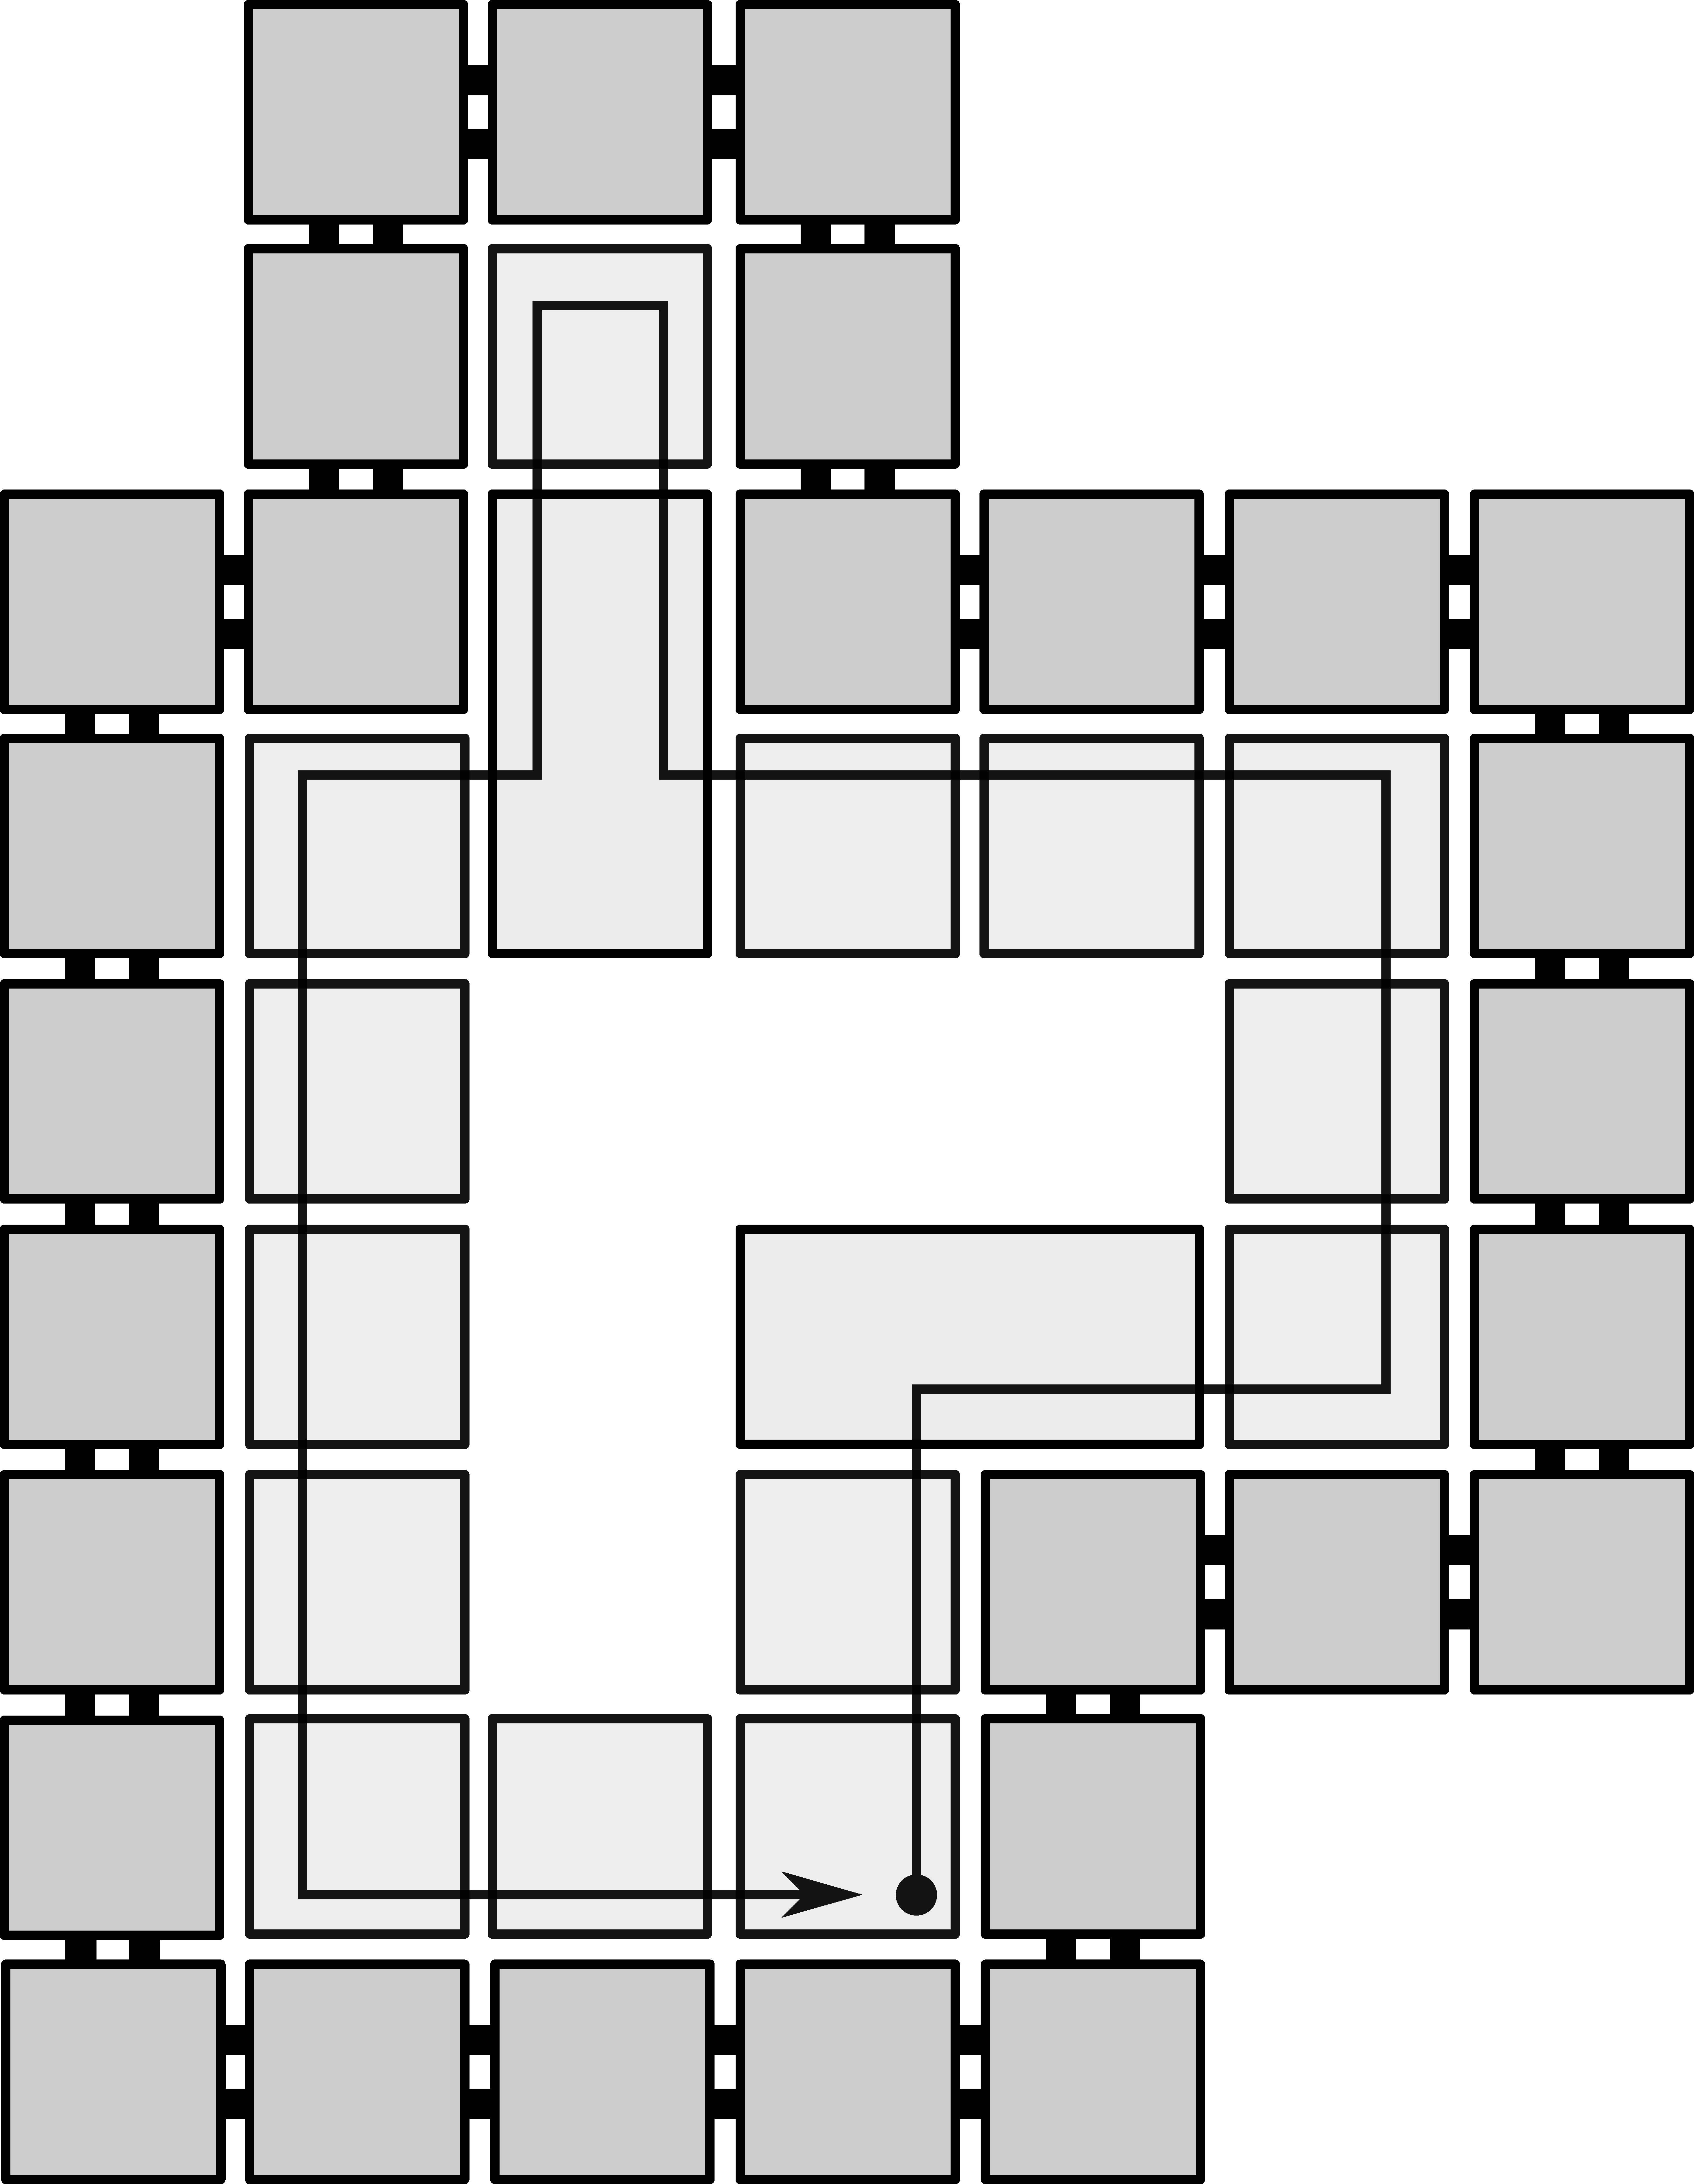
\includegraphics[width=0.6\textwidth]{images/rep_w_examples1.pdf}
  }
  \nocaption{A figure showing one of the steps of shape replication in the STAM.}
  \label{fig:self-assembly-1}
\end{figure}

\begin{figure}
  \centering
  \makebox[\textwidth][c] {
    \includegraphics[scale=.03]{images/3sided-impossible5-2}
  }
  \nocaption{A figure used to show a 3-sided fractal that can grow incorrectly in the 2HAM, hence cannot be strictly self-assembled.}
  \label{fig:self-assembly-2}
\end{figure}

\clearpage
\sectionsubtitle{}
\thispagestyle{plain}
\printbibliography

\end{document}
